% Options for packages loaded elsewhere
\PassOptionsToPackage{unicode}{hyperref}
\PassOptionsToPackage{hyphens}{url}
%
\documentclass[
]{article}
\usepackage{lmodern}
\usepackage{amssymb,amsmath}
\usepackage{ifxetex,ifluatex}
\ifnum 0\ifxetex 1\fi\ifluatex 1\fi=0 % if pdftex
  \usepackage[T1]{fontenc}
  \usepackage[utf8]{inputenc}
  \usepackage{textcomp} % provide euro and other symbols
\else % if luatex or xetex
  \usepackage{unicode-math}
  \defaultfontfeatures{Scale=MatchLowercase}
  \defaultfontfeatures[\rmfamily]{Ligatures=TeX,Scale=1}
\fi
% Use upquote if available, for straight quotes in verbatim environments
\IfFileExists{upquote.sty}{\usepackage{upquote}}{}
\IfFileExists{microtype.sty}{% use microtype if available
  \usepackage[]{microtype}
  \UseMicrotypeSet[protrusion]{basicmath} % disable protrusion for tt fonts
}{}
\makeatletter
\@ifundefined{KOMAClassName}{% if non-KOMA class
  \IfFileExists{parskip.sty}{%
    \usepackage{parskip}
  }{% else
    \setlength{\parindent}{0pt}
    \setlength{\parskip}{6pt plus 2pt minus 1pt}}
}{% if KOMA class
  \KOMAoptions{parskip=half}}
\makeatother
\usepackage{xcolor}
\IfFileExists{xurl.sty}{\usepackage{xurl}}{} % add URL line breaks if available
\IfFileExists{bookmark.sty}{\usepackage{bookmark}}{\usepackage{hyperref}}
\hypersetup{
  pdftitle={SC-2 Electric Boogalo},
  pdfauthor={Kieran Morris, Cecina Babich Morrow and Sherman Kjo},
  hidelinks,
  pdfcreator={LaTeX via pandoc}}
\urlstyle{same} % disable monospaced font for URLs
\usepackage[margin=1in]{geometry}
\usepackage{color}
\usepackage{fancyvrb}
\newcommand{\VerbBar}{|}
\newcommand{\VERB}{\Verb[commandchars=\\\{\}]}
\DefineVerbatimEnvironment{Highlighting}{Verbatim}{commandchars=\\\{\}}
% Add ',fontsize=\small' for more characters per line
\usepackage{framed}
\definecolor{shadecolor}{RGB}{248,248,248}
\newenvironment{Shaded}{\begin{snugshade}}{\end{snugshade}}
\newcommand{\AlertTok}[1]{\textcolor[rgb]{0.94,0.16,0.16}{#1}}
\newcommand{\AnnotationTok}[1]{\textcolor[rgb]{0.56,0.35,0.01}{\textbf{\textit{#1}}}}
\newcommand{\AttributeTok}[1]{\textcolor[rgb]{0.77,0.63,0.00}{#1}}
\newcommand{\BaseNTok}[1]{\textcolor[rgb]{0.00,0.00,0.81}{#1}}
\newcommand{\BuiltInTok}[1]{#1}
\newcommand{\CharTok}[1]{\textcolor[rgb]{0.31,0.60,0.02}{#1}}
\newcommand{\CommentTok}[1]{\textcolor[rgb]{0.56,0.35,0.01}{\textit{#1}}}
\newcommand{\CommentVarTok}[1]{\textcolor[rgb]{0.56,0.35,0.01}{\textbf{\textit{#1}}}}
\newcommand{\ConstantTok}[1]{\textcolor[rgb]{0.00,0.00,0.00}{#1}}
\newcommand{\ControlFlowTok}[1]{\textcolor[rgb]{0.13,0.29,0.53}{\textbf{#1}}}
\newcommand{\DataTypeTok}[1]{\textcolor[rgb]{0.13,0.29,0.53}{#1}}
\newcommand{\DecValTok}[1]{\textcolor[rgb]{0.00,0.00,0.81}{#1}}
\newcommand{\DocumentationTok}[1]{\textcolor[rgb]{0.56,0.35,0.01}{\textbf{\textit{#1}}}}
\newcommand{\ErrorTok}[1]{\textcolor[rgb]{0.64,0.00,0.00}{\textbf{#1}}}
\newcommand{\ExtensionTok}[1]{#1}
\newcommand{\FloatTok}[1]{\textcolor[rgb]{0.00,0.00,0.81}{#1}}
\newcommand{\FunctionTok}[1]{\textcolor[rgb]{0.00,0.00,0.00}{#1}}
\newcommand{\ImportTok}[1]{#1}
\newcommand{\InformationTok}[1]{\textcolor[rgb]{0.56,0.35,0.01}{\textbf{\textit{#1}}}}
\newcommand{\KeywordTok}[1]{\textcolor[rgb]{0.13,0.29,0.53}{\textbf{#1}}}
\newcommand{\NormalTok}[1]{#1}
\newcommand{\OperatorTok}[1]{\textcolor[rgb]{0.81,0.36,0.00}{\textbf{#1}}}
\newcommand{\OtherTok}[1]{\textcolor[rgb]{0.56,0.35,0.01}{#1}}
\newcommand{\PreprocessorTok}[1]{\textcolor[rgb]{0.56,0.35,0.01}{\textit{#1}}}
\newcommand{\RegionMarkerTok}[1]{#1}
\newcommand{\SpecialCharTok}[1]{\textcolor[rgb]{0.00,0.00,0.00}{#1}}
\newcommand{\SpecialStringTok}[1]{\textcolor[rgb]{0.31,0.60,0.02}{#1}}
\newcommand{\StringTok}[1]{\textcolor[rgb]{0.31,0.60,0.02}{#1}}
\newcommand{\VariableTok}[1]{\textcolor[rgb]{0.00,0.00,0.00}{#1}}
\newcommand{\VerbatimStringTok}[1]{\textcolor[rgb]{0.31,0.60,0.02}{#1}}
\newcommand{\WarningTok}[1]{\textcolor[rgb]{0.56,0.35,0.01}{\textbf{\textit{#1}}}}
\usepackage{graphicx}
\makeatletter
\def\maxwidth{\ifdim\Gin@nat@width>\linewidth\linewidth\else\Gin@nat@width\fi}
\def\maxheight{\ifdim\Gin@nat@height>\textheight\textheight\else\Gin@nat@height\fi}
\makeatother
% Scale images if necessary, so that they will not overflow the page
% margins by default, and it is still possible to overwrite the defaults
% using explicit options in \includegraphics[width, height, ...]{}
\setkeys{Gin}{width=\maxwidth,height=\maxheight,keepaspectratio}
% Set default figure placement to htbp
\makeatletter
\def\fps@figure{htbp}
\makeatother
\setlength{\emergencystretch}{3em} % prevent overfull lines
\providecommand{\tightlist}{%
  \setlength{\itemsep}{0pt}\setlength{\parskip}{0pt}}
\setcounter{secnumdepth}{5}

\title{SC-2 Electric Boogalo}
\usepackage{etoolbox}
\makeatletter
\providecommand{\subtitle}[1]{% add subtitle to \maketitle
  \apptocmd{\@title}{\par {\large #1 \par}}{}{}
}
\makeatother
\subtitle{Regression on the Irish datset agregated by class}
\author{Kieran Morris, Cecina Babich Morrow and Sherman Kjo}
\date{}

\begin{document}
\maketitle

{
\setcounter{tocdepth}{3}
\tableofcontents
}
\hypertarget{cleaning-the-data}{%
\section{Cleaning the Data}\label{cleaning-the-data}}

\hypertarget{data-overview}{%
\subsection{Data overview}\label{data-overview}}

We are analyzing a set of Irish household electricity demand available
from the \texttt{electBook} package. We have three datasets:

\begin{itemize}
\tightlist
\item
  \texttt{indCons}: 16799 x 2672 matrix of individual household
  electricity consumption. Each column corresponds to a household and
  each row to a time point. Demand is observed every half hour, so there
  are 48 observations per day per household.
\item
  \texttt{survey}: 2672 row dataframe of household survey data. This
  dataset contains household level data on variables such as social
  class, renting vs.~owning, appliances, etc.
\item
  \texttt{extra}: 16799 row dataframe of time-related variables. This
  dataset contains the date-time of each demand observation, time of
  year, day of week, time of day, whether the day was a holiday, and
  external temperature.
\end{itemize}

\begin{Shaded}
\begin{Highlighting}[]
\CommentTok{\# Extract individual dataframes}
\KeywordTok{library}\NormalTok{(electBook)}
\KeywordTok{library}\NormalTok{(tidyverse)}
\KeywordTok{data}\NormalTok{(Irish)}
\NormalTok{indCons \textless{}{-}}\StringTok{ }\NormalTok{Irish[[}\StringTok{"indCons"}\NormalTok{]]}
\NormalTok{survey \textless{}{-}}\StringTok{ }\NormalTok{Irish[[}\StringTok{"survey"}\NormalTok{]]}
\NormalTok{extra \textless{}{-}}\StringTok{ }\NormalTok{Irish[[}\StringTok{"extra"}\NormalTok{]]}
\end{Highlighting}
\end{Shaded}

\hypertarget{loading-and-structure}{%
\subsection{Loading and Structure}\label{loading-and-structure}}

\begin{Shaded}
\begin{Highlighting}[]
\CommentTok{\# Aggregate total}
\CommentTok{\# Frequency is 30 minutes, so each day has 48 ticks}
\NormalTok{agg \textless{}{-}}\StringTok{ }\KeywordTok{rowSums}\NormalTok{(indCons)}
\end{Highlighting}
\end{Shaded}

\hypertarget{feature-engineering}{%
\subsection{Feature engineering}\label{feature-engineering}}

Based on exploratory data analysis, we created some features from the
dataset to model demand.

\hypertarget{temperature}{%
\subsubsection{Temperature}\label{temperature}}

We can visualize the relationship between temperature and the aggregate
demand over time across all households:

\begin{Shaded}
\begin{Highlighting}[]
\NormalTok{temp\_demand \textless{}{-}}\StringTok{ }\KeywordTok{data.frame}\NormalTok{(}\DataTypeTok{demand =}\NormalTok{ agg) }\OperatorTok{\%\textgreater{}\%}
\StringTok{  }\KeywordTok{bind\_cols}\NormalTok{(Irish[[}\StringTok{"extra"}\NormalTok{]])}

\KeywordTok{ggplot}\NormalTok{(temp\_demand, }\KeywordTok{aes}\NormalTok{(}\DataTypeTok{x =}\NormalTok{ dateTime, }\DataTypeTok{y =}\NormalTok{ demand, }\DataTypeTok{color =}\NormalTok{ temp)) }\OperatorTok{+}
\StringTok{  }\KeywordTok{geom\_point}\NormalTok{() }\OperatorTok{+}
\StringTok{  }\NormalTok{viridis}\OperatorTok{::}\KeywordTok{scale\_color\_viridis}\NormalTok{(}\DataTypeTok{option =} \StringTok{"magma"}\NormalTok{) }\OperatorTok{+}
\StringTok{  }\KeywordTok{labs}\NormalTok{(}\DataTypeTok{x =} \StringTok{"Date"}\NormalTok{, }\DataTypeTok{y =} \StringTok{"Total Demand"}\NormalTok{, }\DataTypeTok{color =} \StringTok{"Temperature"}\NormalTok{) }\OperatorTok{+}
\StringTok{  }\KeywordTok{theme\_bw}\NormalTok{()}
\end{Highlighting}
\end{Shaded}

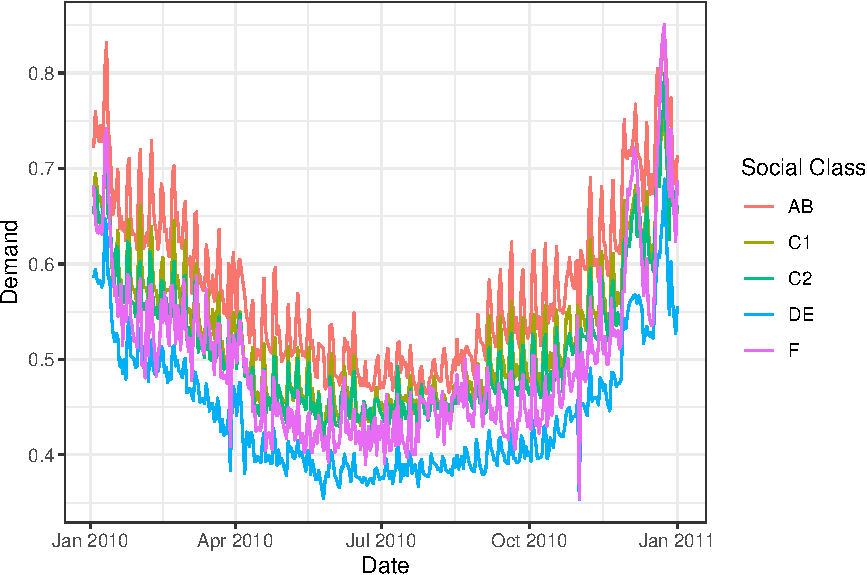
\includegraphics{main_files/figure-latex/unnamed-chunk-3-1.pdf}

We can see that during the warmer summer months, demand dips, although
the pattern is messy. We included linear and quadratic terms for
temperature in our models.

\hypertarget{day-of-the-week}{%
\subsubsection{Day of the week}\label{day-of-the-week}}

Since we have the categorical variable day of the week for each date, we
used one-hot encoding to include this information in our models.

\hypertarget{fourier-terms}{%
\subsubsection{Fourier terms}\label{fourier-terms}}

We used Fourier terms to capture the patterns of seasonality in the
data. Fourier terms are a set of sine and cosine functions with
different frequencies that can be used to model periodic patterns. For a
given period \(P\), the Fourier terms are defined as follows:
\[\text{sin}_k(t) = \sin\left(\frac{2\pi kt}{P}\right), \quad \text{cos}_k(t) = \cos\left(\frac{2\pi kt}{P}\right)\]
where \(k\) is the frequency and \(t\) is the time.

We used Fourier terms to model the daily and annual seasonality in the
data.

\hypertarget{social-class}{%
\subsection{Social class}\label{social-class}}

We wanted to investigate demand patterns across different social
classes. The dataset includes 5 social classes, defined by the
occupation of the head of household:

\begin{itemize}
\tightlist
\item
  AB: managerial roles, administrative or professional
\item
  C1: supervisory, clerical, junior managerial
\item
  C2: skilled manual workers
\item
  DE: semi-skilled and unskilled manual workers, state pensioners,
  casual workers
\item
  F: farmers
\end{itemize}

** Insert plot of demand patterns for different classes **

We modeled the average demand for each social class separately.

\hypertarget{simple-regression}{%
\section{Simple Regression}\label{simple-regression}}

\hypertarget{theory}{%
\subsection{Theory}\label{theory}}

\hypertarget{model}{%
\subsection{Model}\label{model}}

\hypertarget{implementation}{%
\subsection{Implementation}\label{implementation}}

\hypertarget{ridge-regression}{%
\section{Ridge Regression}\label{ridge-regression}}

\hypertarget{theory-1}{%
\subsection{Theory}\label{theory-1}}

Ridge regression is a method for penalized regression. Consider the
model \[Y_i^0 = \alpha + \beta x_i^0 + \epsilon_i, \quad  i = 1,..., n\]
where \(\beta \in \mathbb{R}^p\), \(\alpha \in \mathbb{R}\), and for all
\(i, l \in \{1, ..., n\}\), \(\mathbb{E}[\epsilon_i] = 0\) and
\(\mathbb{E}[\epsilon_i \epsilon_l] = \sigma^2 \delta_{il}\) for some
\(\sigma^2 > 0\). Then the ridge regression estimator is defined as the
minimizer of the following objective function:
\[(\hat{\alpha}_\lambda, \hat{\beta}_\lambda) = \mathrm{argmin}_{\alpha \in \mathbb{R}, \beta \in \mathbb{R}^p} \lVert y^0 - \alpha - \boldsymbol{X}^0 \beta \rVert^2_2 + \lambda \lVert \beta \rVert^2_2\]
where \(\lambda > 0\) is a tuning parameter and
\(\lVert \cdot \rVert_2\) denotes the Euclidean norm. Ridge regression
is thus imposing a penalty on the size of \(\beta\), with the strength
of that penalty determined by the choice of \(\lambda\). The
coefficients will be shrunk towards zero, but will not be set to zero
(as opposed to in lasso regression).

\hypertarget{model-1}{%
\subsection{Model}\label{model-1}}

\hypertarget{implementation-1}{%
\subsection{Implementation}\label{implementation-1}}

\hypertarget{gaussian-process-regression}{%
\section{Gaussian Process
Regression}\label{gaussian-process-regression}}

\hypertarget{theory-2}{%
\subsection{Theory}\label{theory-2}}

A gaussian process is a collection of random variables, which have a
joint Gaussian distribution. A Gaussian process is completely specified
by its mean function and covariance function. We build the following
model:

Let \(y_i = f(x_i) + \varepsilon_i\), where
\(f(x) \sim \text{GP}(0, k(x, x'))\) and
\(\varepsilon_i \sim N(0, \sigma^2)\). Then we can find the posterior
distribution of \(f(x_*)\) given \(y\) as:

\[
f(x_*) | y \sim N(\mu(x_*), \sigma^2(x_*))
\]

where \(\mu(x_*) = k(x_*, x)^T(K + \sigma^2I)^{-1}y\) and
\(\sigma^2(x_*) = k(x_*, x_*) - k(x_*, x)^T(K + \sigma^2I)^{-1}k(x_*, x)\).
In pratice, to find the posterior distribution, we maximise the marginal
log-likelihood.

\hypertarget{model-2}{%
\subsection{Model}\label{model-2}}

\hypertarget{implementation-2}{%
\subsection{Implementation}\label{implementation-2}}

\hypertarget{results}{%
\section{Results}\label{results}}

\end{document}
